\documentclass{article}

% if you need to pass options to natbib, use, e.g.:
% \PassOptionsToPackage{numbers, compress}{natbib}
% before loading nips_2016
%
% to avoid loading the natbib package, add option nonatbib:
% \usepackage[nonatbib]{nips_2016}

% \usepackage{nips_2016}

% to compile a camera-ready version, add the [final] option, e.g.:
\usepackage[final]{nips_2016}

\usepackage[utf8]{inputenc} % allow utf-8 input
\usepackage[T1]{fontenc}    % use 8-bit T1 fonts
\usepackage{hyperref}       % hyperlinks
\usepackage{url}            % simple URL typesetting
\usepackage{booktabs}       % professional-quality tables
\usepackage{amsfonts}       % blackboard math symbols
\usepackage{nicefrac}       % compact symbols for 1/2, etc.
\usepackage{microtype}      % microtypography
\usepackage{graphicx}
\usepackage{amsmath, amsfonts}
\usepackage{dsfont}


\title{10807 Topics in Deep Learning HW1}

% The \author macro works with any number of authors. There are two
% commands used to separate the names and addresses of multiple
% authors: \And and \AND.
%
% Using \And between authors leaves it to LaTeX to determine where to
% break the lines. Using \AND forces a line break at that point. So,
% if LaTeX puts 3 of 4 authors names on the first line, and the last
% on the second line, try using \AND instead of \And before the third
% author name.

\author{
  Erik Sjoberg\\
  esjoberg\\
  School of Computer Science\\
  The Robotics Institute\\
  \texttt{esjoberg@cmu.edu} \\
  %% examples of more authors
  %% \And
  %% Coauthor \\
  %% Affiliation \\
  %% Address \\
  %% \texttt{email} \\
  %% \AND
  %% Coauthor \\
  %% Affiliation \\
  %% Address \\
  %% \texttt{email} \\
  %% \And
  %% Coauthor \\
  %% Affiliation \\
  %% Address \\
  %% \texttt{email} \\
  %% \And
  %% Coauthor \\
  %% Affiliation \\
  %% Address \\
  %% \texttt{email} \\
}

\begin{document}
% \nipsfinalcopy is no longer used

\maketitle

\begin{abstract}
  Simple implementation of backpropagation in a fully connected neural network.
\end{abstract}

\section{Overfitting and Model Complexity}

\subsection{Typical Training Behavior: Error Rate vs Model Complexity}
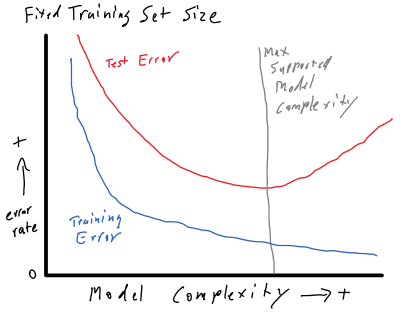
\includegraphics[scale=0.6]{error_vs_modelcomplexity.png} 

\subsection{Typical Training Behavior: Error Rate vs Training Set Size}
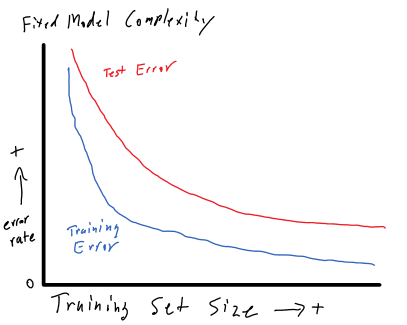
\includegraphics[scale=0.6]{error_vs_trainsetsize.png} 


\section{Expected Loss for Regression}

\subsection{a) Case q = 1}
Starting with 
\begin{gather}
E \left[ { L }_{ q } \right] =\int { \int { { |y(x) - t| }^{ q }p(x,t)dtdx }  } 
\end{gather}
using the independence of our choice of y(x) every point x, we can simplify this for the purposes of minimization to the following:
\begin{gather}
E \left[ { L }_{ q } \right] = \int { { |y(x) - t| }^{ q }p(t|x)dt }
\end{gather}
For the case q=1, the both sides of the integral around y(x) have linearly increasing weight, and the minimum is reached when this linear valley is centered on the average of the distribution of density.

With Q=1, taking the directional derivative of the above with respect to y(x) and setting it equal to zero gives
\begin{gather}
\int _{-\infty}^{y(x)} {p(t|x)dt } - \int _{y(x)}^{\infty} {p(t|x)dt } = 0
\end{gather}

Which is the same as saying that the expectation corresponds to the conditional median. 

\subsection{b) Case q -> 0}

In the case of the limit where q approaches 0, the distribution becomes equal to 1 everywhere except for an infinitely narrow valley right above $y(x)=t$.

Therefore, the expected loss will be minimized when this valley is directly above the point of the function with the highest probability density.  This corresponds to the conditional mode. 


\section{Binary Classification Error Function}

We know that for general binary classification, the cross-entropy loss function takes the form $l=-\sum c_i\log(p_i)$ where $c_i$ is the class indicator. This corresponds to the negative log likelihood. 

If there is a probability $\epsilon$ that a class label is wrong, we can say that 
\[
p_i=\epsilon/N + (1-\epsilon)y_i
\]
where N is the total number of classes, 2 in this case. 

The error function then becomes:
\[
l=-\sum c_i\log(\epsilon/2 + (1-\epsilon)y_i)
\]




\section{Generalized Gaussian}

\subsection{Show Distribution is Normalized}
Starting with the generalized Gaussian below, 
\[
P(x)=\frac { q }{ {2(2 \sigma ^{2})^{1/q}  } \Gamma (1/q) } exp(- \frac {|x|^{q}}{2\sigma^{2}})  
\]
first see that when q = 2, it can be shown that $\Gamma(1/2) = \sqrt{\pi}$ and $(2\sigma^{2})^{1/2} = \sigma \sqrt{2}$. Canceling the 2 from the top and bottom of the left side, brings us back to the familiar left-hand form of the gaussian:
\[
P(x) = \frac{1}{{\sigma \sqrt {2\pi } }}e^{{{ - \left( {x - \mu } \right)^2 } \mathord{\left/ {\vphantom {{ - \left( {x - \mu } \right)^2 } {2\sigma ^2 }}} \right. \kern-\nulldelimiterspace} {2\sigma ^2 }}}
\]

This generalized distribution can be shown to be properly normalized (adds up to one) with the knowledge that the following equation holds in the eve more general case where x is not restricted to be positive.  
\begin{gather}
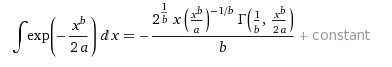
\includegraphics[scale=1]{big_integral.png} 
\end{gather}

When x is positive, as in our example above, the second gamma term is redundant and this factor perfectly cancels out the remaining terms of our original generalized Gaussian. 

\subsection{Derive Log-likelihood Function}
The derivation of the log-likelihood function can proceed as follows
\[
L(q, \sigma,x_1, ..., x_n)=\prod _{ j=1 }^{ n }{   \frac { q }{ { 2(2\sigma ^{ 2 })^{ 1/q } }\Gamma (1/q) } exp(-\frac { |x_{j}|^{ q } }{ 2\sigma ^{ 2 } } )}
\]
\[
L(q,\sigma ,x_{ 1 },...,x_{ n })=\frac { q }{ { 2(2\sigma ^{ 2 })^{ 1/q } }\Gamma (1/q) } exp(- 1/2\sigma^2\sum _{ j=1 }^{n  }{   |x_{ j }|^{ q } } )
\]
\[
log(L(q,\sigma ,x_{ 1 },...,x_{ n })) = ln(\frac { q }{ { 2(2\sigma ^{ 2 })^{ 1/q } }\Gamma (1/q) } ) +ln(exp(- 1/2\sigma^2\sum _{ j=1 }^{n  }{   |x_{ j }|^{ q } } ))
\]
\[
log(L(q,\sigma ,x_{ 1 },...,x_{ n })) = ln(\frac { q }{ { 2(2\sigma ^{ 2 })^{ 1/q } }\Gamma (1/q) } ) - \frac{1}{2\sigma^2}\sum _{ j=1 }^{n  }{   |x_{ j }|^{ q } } 
\]



\section{Implementation of Backpropagation}

\subsection{a) Basic Generalization}
The red lines in Figure \ref{fig:crosen1} shows test-set performance across 200 epochs, while the blue lines show the train-set performance. The network was trained 5 times with different seeds each time, with a learning rate of 0.1.  

\begin{figure}[h]
  \centering
  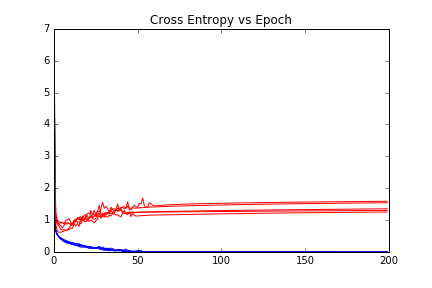
\includegraphics[scale=0.6]{../5a_crossentropy_vs_epoch_200.png} 
  \caption{Training cross-entropy error (blue) and test cross-entropy error (red) for 5 seeds.}
  \label{fig:crosen1}
\end{figure}

It is clear that the performance is significantly different on the test set versus the training set.  With this learning rate, the network achieves it's best test-set performance after only 10 epochs, after which the cross-entropy of the test-set starts to rise. In contrast, the train-set cross-entropy performance continues to decrease for up to around 60 epochs before leveling out. The validation curve clearly shows a different behavior.


\subsection{b) Classification Error}

Figure \ref{fig:class1} shows the test and train set performance as measured by the classification error across 200 epochs.  The behavior of the classification training error is clearly different from that of the cross entropy test error: the classification error never actually increases as training progresses, in contrast with the cross entropy error which did rise (as expected) as training progressed. 

\begin{figure}[h]
  \centering 
  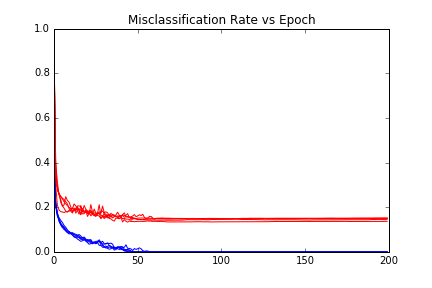
\includegraphics[scale=0.6]{../5b_misclassification_vs_epoch_200.png} 
  \caption{Training classification error (blue) and test classification error (red) for 5 seeds.}
  \label{fig:class1}
\end{figure}

This suggests that cross-entropy may do a better job than classification error of indicating when over-fitting is taking place. 


\subsection{c) Visualizing Parameters}

Figure \ref{fig:paramviz} shows a good amount of structure in the learned parameter W from the bottom level of the network. Curves, edges, and lines reminiscent of numbers and parts of numbers can be seen. 

This visible structure is suggestive that the backpropagation is working, and the network is learning generalized structure from the data. 

\begin{figure}[h]
  \centering
  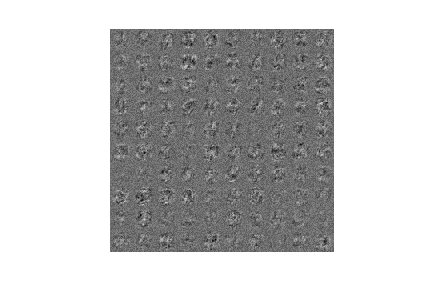
\includegraphics[scale=0.7]{../5c_parameter_viz.png} 
  \caption{Visualization of 10-by-10 grid of learned parameters from the bottom layer of the network.}
  \label{fig:paramviz}
\end{figure}

\subsection{d) Learning Rate}

For my implementation, I found that the performance with lower learning rates is significantly better than higher learning rates as can be see in Figure \ref{fig:learnrates}.  The convergence of test and training performance is far more similar with a rate of 0.01 as compared to 0.1 or 0.2.  With a learning rate of 0.5, no learning appears to take place whatsoever. 
\begin{figure}[h]
  \centering
  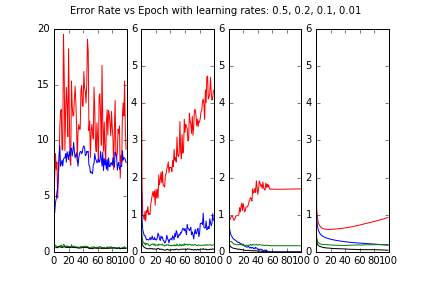
\includegraphics[scale=0.6]{../learning_rates.png} 
  \caption{Visualization of error rates with various learning rates. Red and blue are cross-entropy error for test and train, while green and black are categorization error for test and train respectively. }
  \label{fig:learnrates}
\end{figure}

Figure \ref{fig:momentums} also shows interesting behavior, with the network training significantly better in the absence of momentum. With large momentum, even the train error (blue) fails to converge, showing a U shape. Absolute values of both error functions are also better with minimal momentum. This may be due to the usage of mini-batch size one (gradient updates occur after every training sample). 

\begin{figure}[h]
  \centering
  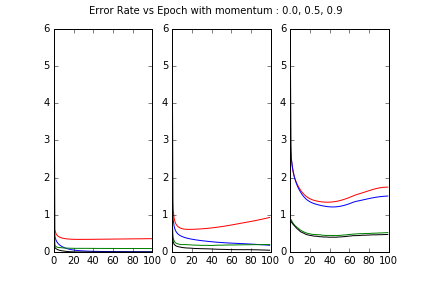
\includegraphics[scale=0.6]{../momentum_tests.png} 
  \caption{Visualization of error rates with various momentum values. Red and blue are cross-entropy error for test and train, while green and black are categorization error for test and train respectively. }
  \label{fig:momentums}
\end{figure}

To choose the best parameters, it is clearly necessary to test them empirically, perhaps performing a grid-search over promising candidate parameter sets. In this case, I would lean towards low or no momentum, as well as a low learning rate to encourage stability when training with mini-batch size equal to 1.

\subsection{e) Number of Hidden Units}

Varying the number of hidden units, as seen in Figure \ref{fig:hiddenunits}, has an interesting effect on the error rates as training progresses.  In all cases, higher hidden layer counts resulted in progressively decreased train-set error, as well as faster convergence to those lower values. 

On the other hand, overfitting was a problem for networks with more hidden units as would be expected. The test-set errors (red line) can be seen to grow significantly more quickly with the networks trained with 200 and 500 hidden units. 

It looks like the current setting of 100 hidden units was a sweet spot, as this setting achieved the lowest classification error among all three (0.165 vs as high as 0.211) These networks were trained with rate=0.01 and momentum=0.5, which in contrast to the default setting of hidden layers appears to be a sub-optimal setting for this network. 

\begin{figure}[h]
  \centering
  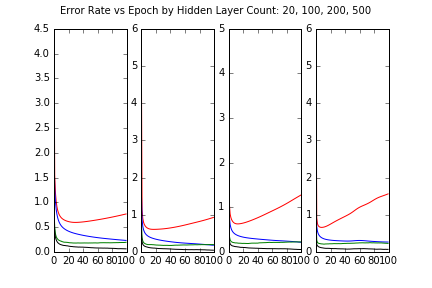
\includegraphics[scale=0.6]{../hidden_units.png} 
  \caption{Visualization of error rates with various numbers of hidden layers. Red and blue are cross-entropy error for test and train, while green and black are categorization error for test and train respectively. }
  \label{fig:hiddenunits}
\end{figure}

\subsection{f) Dropout}



\begin{figure}[h]
  \centering
  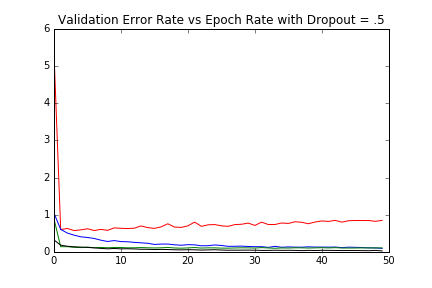
\includegraphics[scale=0.6]{../dropout1.png} 
  \caption{Visualization of error rates during training with dropout. Red and blue are cross-entropy error for test and train, while green and black are categorization error for test and train respectively. }
  \label{fig:momentumsrate1}
\end{figure}


\subsection{g) Best-Performing Single Layer}

After exploring a wide range of parameter values over the previous sections, it became clear that a learning rate of 0.05, momentum of 0, and a layer size of 100 is the best performing combination for this code, achieving a minimum validation error of 7.9/%.  


\begin{figure}[h]
  \centering
  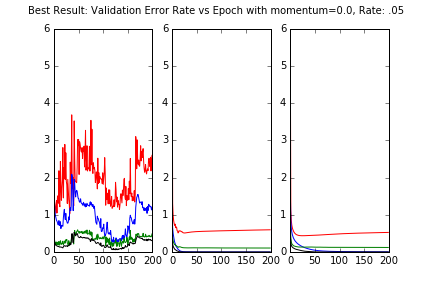
\includegraphics[scale=0.6]{../one_layer_best.png} 
  \caption{Visualization of error rates of the single-layer network with the best performance. Red and blue are cross-entropy error for test and train, while green and black are categorization error for test and train respectively. }
  \label{fig:momentumsrate1}
\end{figure}


\subsection{h) Extension to Multiple Layers}

When training a network with multiple hidden layers (two in this case), it was interesting to note that less over-fitting was observed on the test set during training out to 200 epochs for most standard settings.  This was a bit unexpected, since the network with more layers has more capacity to fit a model.  It may be that this is reflecting the. 

To evaluate the performance of the network, a 9-cell grid-search over 3 values each of momentum and learning rate was carried out, as can be seen in Figure \ref{fig:momentumsrate1}, \ref{fig:momentumsrate2} and \ref{fig:momentumsrate3}. Momentum varied between 0.0, 0.2, and 0.5, while learning rate varied between 0.1, 0.05, and 0.01. During this training dropout was 0, and hidden-layer count was 100. 

The best performer was the test with momentum at 0 and learning rate at 0.05, achieving a classification error of 8.9\% at around epoch 10. 	 

\begin{figure}[h]
  \centering
  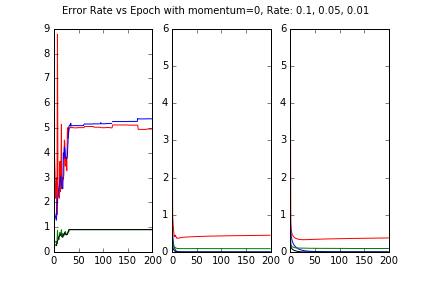
\includegraphics[scale=0.6]{../momentum0_rate10501.png} 
  \caption{Visualization of error rates with various momentum values. Red and blue are cross-entropy error for test and train, while green and black are categorization error for test and train respectively. }
  \label{fig:momentumsrate1}
\end{figure}



\begin{figure}[h]
  \centering
  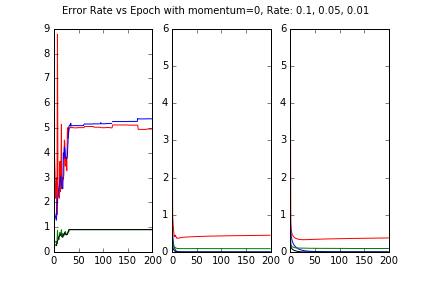
\includegraphics[scale=0.6]{../momentum0_rate10501.png} 
  \caption{Visualization of error rates with various momentum values. Red and blue are cross-entropy error for test and train, while green and black are categorization error for test and train respectively. }
  \label{fig:momentumsrate2}
\end{figure}

\begin{figure}[h]
  \centering
  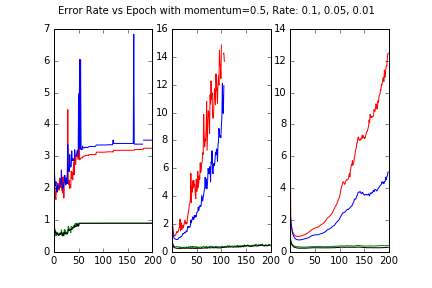
\includegraphics[scale=0.6]{../momentum5_rate10501.png} 
  \caption{Visualization of error rates with various momentum values. Red and blue are cross-entropy error for test and train, while green and black are categorization error for test and train respectively. }
  \label{fig:momentumsrate3}
\end{figure}

\begin{figure}[h]
  \centering
  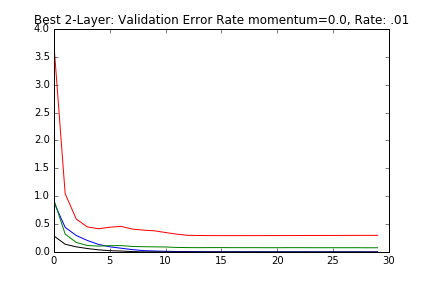
\includegraphics[scale=0.6]{../two_layer_best.png} 
  \caption{Visualization of VALIDATION error rates for the best two-layer network. Red and blue are cross-entropy error for test and validation, while green and black are categorization error for test and validation respectively. }
  \label{fig:twolayerbest}
\end{figure}




\end{document}
